\begin{flushleft}
    \section{Analysis} 
        \subsection{Statment Of Problem}
        \large
        \bk
        Maps, as you would think of them today, have been arround since 6\textsuperscript{th} century BC and since then have been in constant use by people in their day to day lives. 
        The more modern version of maps, for example Google maps or Bing maps have only been around since the late 1990's. The problem that I am going to be solving is map pathfinding.
        Currently not all roads and paths are logged and entered into a searchable format. The only way some people have to navigate terrain is through the use of old style paper maps.
        The problem with paper maps is that they are not easily, at a glance, used to find a path from point to point. As well as this sometimes are not easy to comprehend just by looking 
        at them with various terrain features. \\
        
        \bk
        \begin{figure}[h]
            \centering
            \subfloat[\centering Map without labeles on roads]{{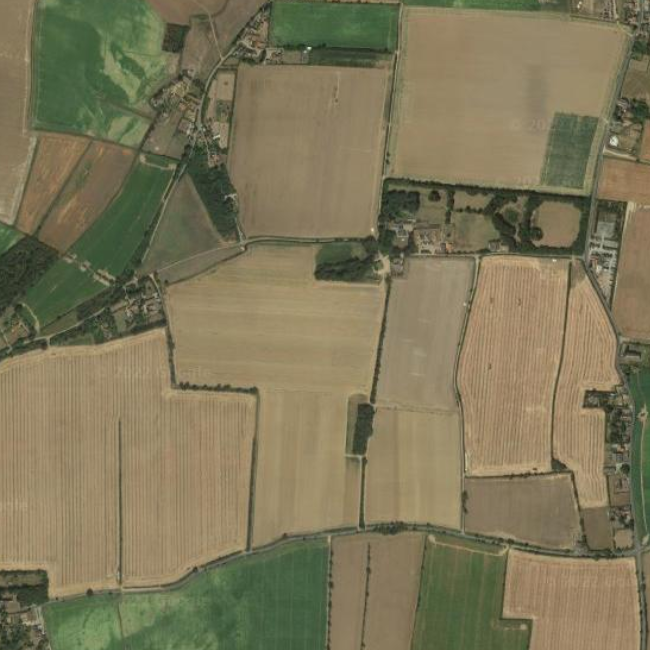
\includegraphics[width=6cm]{images/unlabeledMap.png}}}
            \qquad
            \subfloat[\centering Map with labeles on roads]{{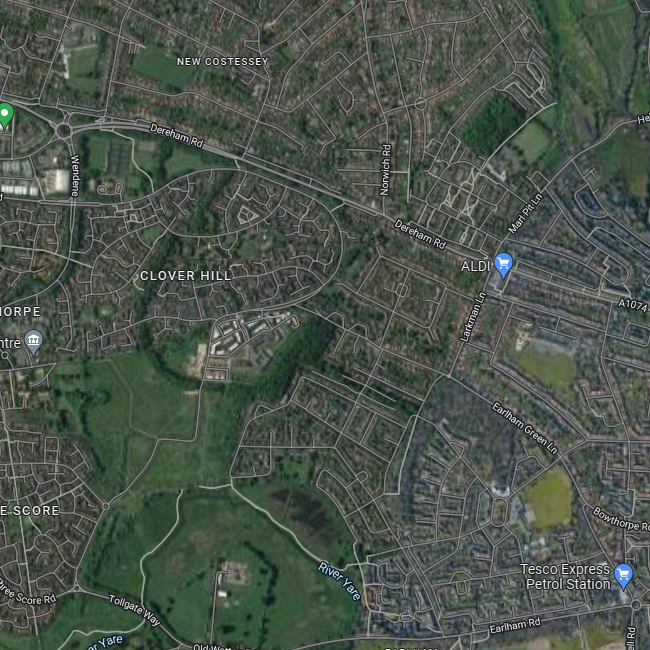
\includegraphics[width=6cm]{images/labeledMap.png}}}
            \caption*{Examples of maps with and without lables taken from Google Maps\textsuperscript{\textcopyright}}
        \end{figure}
        \bk

        This can cause issues for people who live out in areas which have not been mapped. This is because they cannot create easy to follow routes with the click of a button. Therefor, 
        causing people who live in rural areas to waste time getting used to the routes they have to take to go anywhere. Overall, the problem I am going to be creating a solution for is 
        how people are unable to easily go from point to point at the click of a button and be easily able to, at a glance, interpret the map without prior expeirence. \\

        \subsection{Background}
        \bk
        When people ussualy want to go about planning a journy they will use a service, for example Google Maps to get from one location to another. This usually takes the form of clicking 
        a location and then selecting an origin. This isn't always possible however, this can be for a multitude of reasons it seems however I will briefly go over some below:\\
        
        \begin{enumerate}
            \item \textbf{Either the destination or origin location(s) are not in the service's database.}
            \item \textbf{The destination and origin have no clear defined path between them.}
            \item \textbf{Either the destination or origin are off any predefined track.}
            \item \textbf{The travel method the user has selected is not able to traverse the terrain between the origin and destination.}
        \end{enumerate}

        \bk
        Some of these I beleive are out of the scope of this project however once the interview has been conducted with the end user I will have a better idea of the needs that my program needs to forfill.\\

        \bk
        Finally, 

        \bk
        
        \subsection{End User}
            \subsubsection{First Interview}
            \lipsum[2]
            
            \subsubsection{Evaluation of First Interview}
            \lipsum[2]

        \bk

        \subsection{Initial Research} 
            \subsubsection{Existing Solutions}
            \lipsum[2]

            \subsubsection{Possible Algorithmic Solutions}
            \lipsum[2]

            \subsubsection{Key Components Required}
            \lipsum[2]

        \subsection{Further Research}
            \subsubsection{Algorithmic Deep Dive}
            \lipsum[2]

            \subsubsection{Second Interview}
            \lipsum[2]

            \subsubsection{Evaluation of Second Interview}
            \lipsum[2]

        \subsection{Objectives}
            \lipsum[2]

        \subsection{Modeling}
            \lipsum[2]

        \bk

\end{flushleft}